\chapter{Materiais e Métodos}

Neste capítulo apresenta-se os métodos experimentais utilizados para 
quantificação das concentrações de massa total, das espécies químicas e 
do Black Carbon nas amostras. Empregou-se, respectivamente:
Análise gravimétrica, Fluorescência de raios X (XRF),
Thermal/Optical Transmittance (TOT) e Refletância.
Apresenta-se sinteticamente o desenvolvimento teórico de cada método, bem como 
as condições de uso, procedimentos de calibração, cálculo das incertezas, 
vantagens e desvantagens, entre outros.

Para resolução dos modelos receptores, expõe-se também os métodos 
estatísticos Análise de Fatores e Positive Matrix Factorizarion (PMF) 
usados na identificação dos perfis de fontes. 

Desensolve-se ainda, uma metodologia para estimativa das incertezas
da calibração da XRF e Refletância, fundamentais para análises de PMF,
cuja metodologia emprega a ponderação pelas incertezas.

%%%%
\section{Amostragem}
%TODO: citar artigo do harvardinho (Impactor Desing)
% http://maps.google.com/maps/ms?ie=UTF8&hl=en&msa=0&msid=116003586198857296821.00046d7e7367b947abe12&z=12

Foram coletadas, entre Novembro de 2006 e Agosto de 2008, 858 amostras válidas, 
de 48 horas, em dois sítios de \textbf{Nima}, sendo um localizado perto da rodovia
(+5° 34' 54.00", -0° 11' 56.30") e outro parte residencial do 
bairro (+5° 35' 2.00", -0° 11' 58.80").

A coleta foi diária, mas houve dias sem coleta devido a falta de eletricade e
filtros danificados no transporte ou na troca no amostrador. 
O tempo de amostragem de 48 horas, foi definido antes da entrada \textbf{USP} 
no projeto e trouxe dificuldades nas análises multivaridas, pois o
ciclo de 48h para a amostragem dificulta a captação das especificidades 
de cada uma das fontes.

As amostras de foram coletadas em filtro de teflon do tipo 
\textbf{PTFE} de 37 $mm$ de diâmetro orifícios de 0,2 $\mu m$ de diâmetro. 

Para $MP_{10}$ utilizou-se impactador Harvard com $D_{50}$ de $10 \mu m$ 
com fluxo de $10,0 L/min$ \citep{marple1987}. 
Nas medidas de $MP_{2,5}$, também utilizou-se impactador Harvard, 
mas com $D_{50}$ de $2,5 \mu m$ acoplado com um \textbf{inlet} 
responsável fazer a filtragem de $MP_{2,5}$.

Filtros brancos de campo e laboratórios foram separados para avaliar 
possíveis contaminações no tranporte e manipulação das amostras. 

O laboratório da \textbf{Harvard School of Public Health} foi
utilizada para pesagem das amostras.
Os filtros foram pesados antes e depois da coleta, usando uma balança 
microanalítica \textbf{(Mettler Toledo MT5)} com precisão de $1 \mu g$, 
seguindo procedimentos padrões de controle de umidade ($39 \pm 2 \%$), 
temperatura ($20,5 \pm 0,2 ^{\circ} C$) e eliminação de cargas eletrostáticas 
(fonte de polônio).
Cada pesagem foi realizada duas vezes e o valor final foi a média das 
duas medidas.

As concentrações foram calculadas a partir dos volumes 
medidos por um integrador de volume.


I confirmed with Jose Vallarino who provided
>>>>certain uncertainty parameters to EPA.
>>>>
>>>>1) 5\% flow rate uncertainty is a standard value used here (HSPH).
>>>>2) 6.7 sq.cm for 37-mm filters with
>>>>uncertainty 0.134 sq.cm is a standard value
>>>>measured in HSPH. However, Jose said the
>>>>sample deposit area uncertainty
>>>>measured/calculated by you might be better since you used an SEM.
>>>>3) We did not provide monitor correction, my
>>>>best guess is they did not use it.
>>>> 

>>  I believe this is a standard number used
>>>>> by EPA. EPA use 10.65 sq.cm
>>>>> for 47-mm filters, 6.7 sq.cm for 37-mm filters.
>>>>>
>>>>>  The filter deposition area uncertainty of
>>>>> 37-mm filters is 0.134 sq.cm. I could confirm this with them 




%%%%
\newpage
\section{Fluorescência de Raios X}

Para quantificar a composição elementar (10 < Z < 83) das 
amostras foi utilizada a técnica não-destrutiva de Fluorescência de Raios X 
(XRF), um método analítico quali-quantitativo, multielementar, 
que mede os raios X característicos emitidos pelos átomos da amostra, 
depois de também serem excitados por raios X. Permite análise simultânea dos 
elementos químicos e não exige pré-tratamento dos alvos.

Há basicamente três etapas envolvidas na técnica de medida de raios X 
característicos: excitação da amostra, emissão de raios X pelos átomos da amostra
e detecção. A excitação pode ocorrer por feixe de raios X (ou raios gamas) 
produzido em fontes radioativas, por partículas aceleradas 
(elétrons, prótons, alfas etc) ou 
por tubos geradores de raios X quando submetidos a diferença de potencial
\citep{jenkins1988}.

No caso da XRF, a excitação ocorre por um feixe de raios X incidente, que  
expulsa os elétrons das camadas mais internas do átomo (K, L e M) 
produzindo vacâncias. Para tal, a energia do feixe incidente deve ser maior 
que a energia de ligação dos elétrons nessas camadas. Um átomo com vacância é 
instável e rapidamente elétrons das camadas mais externas preenchem as vacâncias,
liberando fotóns e estabilizando o átomo, sendo a energia destes fótons 
correspondentes às energias de transição entre camadas do átomos, 
característica de cada elemento químico. O processo de excitação do átomo 
é ilustrado classicamente na figura \ref{fig:shimadzu_atomo}.

\begin{figure}[H]
  \centering
  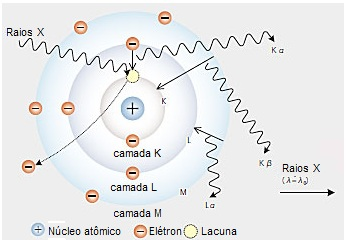
\includegraphics[width=0.5\textwidth]{../inputs/images/shimadzu_atomo.jpg}
  \caption{Ilustração clássica do fenômeno de fluorescência de raios X no átomo. 
           Figura que acompanha o manual da Shimadzu da série de equipamentos
           EDX 700. \label{fig:shimadzu_atomo}}
\end{figure}

As transições dos elétrons entre os níveis quânticos K, L e M encontram-se 
tipicamente na faixa dos raios X, tendendo a ultravioleta (UV) e luz visível,
conforme ocorram em transições atômicas de menor energia no átomo.

Transições da camada L para K são do tipo $K_{\alpha}$, de M para K 
são $K_{\beta}$ e de M para L são $L_{\alpha}$ ou $L_{\beta}$. 
As camadas L e M possuem ainda subníveis de energia, o que resulta em diversas
combinações de transições, sendo algumas delas proibidas, e outras 
com diferenças de energia indistinguíveis para os detectores utilizados 
neste método analítico (XRF-ED).

As principais transições possíveis estão sintetizada na figura \ref{fig:siegbahn}, 
segundo a notação desenvolvida por Siegbahn \citep{jenkins1991}. A referida 
notação, permite identificar melhor os subníveis de origem e destino, por exemplo, 
a transição de $M_{IV}$ para $L_{III}$ é uma transição do tipo $L_{\beta_1}$. 

\begin{figure}[H]
  \centering 
  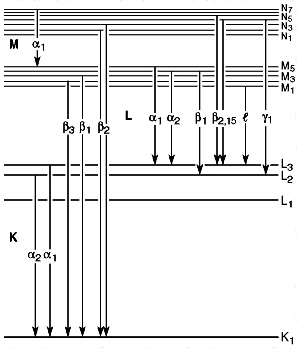
\includegraphics[width=0.5\textwidth]{../inputs/images/Siegbahn.jpg}
  \caption{Transições de elétrons entre os subníveis das camadas K, L e M. 
           Figura extraída de \citet{jenkins1991}. \label{fig:siegbahn}}
\end{figure}

Na prática, dependendo do modo de detecção dos raios X, agrupa-se transições 
dos subníveis e trabalha-se com as denominações de linhas K e L apenas. As linhas
$K_{\alpha}$ são as mais intensas, oferecendo melhor limite de detecção
para um elemento, mas quando muito energéticas, podem ultrapassar a
faixa de sensibilidade do detector empregado. Nestes casos as linhas L passam a 
ser analisadas. No modelo de XRF usado nesta pesquisa, analisou-se as linhas K, 
desde o sódio (Na) até o nióbio (Nb), e as linha L, do molibdênio (Mo) até o chumbo (Pb).  
 
%%%%
\subsection{Tipos de XRF}

Há essencialmente dois tipos principais de equipamentos de XRF que se 
diferenciam pelo modo como os raios X são detectados: fluorescência de raios 
X dispersivo em comprimento de onda (XRF-WD) e fluorescência de raios X 
dispersivo em energia (XRF-ED).

Na XRF-WD os raios X da amostra sofrem difração em um cristal, quantificando-se
os elementos químicos pela contagem de fótons nos ângulo de difração $\theta$, 
característicos dos elementos, segundo a lei de Bragg:

\begin{equation}
	\label{eq:bragg}
	2d sen(\theta) = n \lambda
\end{equation}

Onde, $d$ é 1a distância entre planos do cristal, $\theta$ o ângulo de incidência 
em relação ao plano considerado, $\lambda$ o comprimento de onda 
(e, portanto, a energia) da radiação incidente e $n$ um inteiro.
Esse tipo de equipamento permite uma grande resolução dos comprimentos de onda 
(energia) característicos dos elementos, facilitando detectá-los e, geralmente, 
com bom limite de detecção (LD).
Entretanto, apresentam diversos problemas práticos quando empregados em filtros 
de aerossol atmosférico. Em função disso há uma preferência pelos sistemas 
dispersivos em energia nesse campo de análise. 

A XRF-ED usa detectores de semicondutores capazes de discriminar energias 
próximas com alta resolução temporal, viabilizando a detecção simultânea dos 
elementos químicos através da amplitude do pulso eletrônico produzido no 
detector, proporcional à energia do fóton incidente. O sistema eletrônico do 
equipamento faz a conversão analógica-digital da intensidade do pulso, 
acumulando a contagem por energia em um multicanal. O detector mais empregado é 
o de silício ativado com lítio Si(Li). 

Neste sistema, o LD das análises é particularmente limitado pelos raios X de 
excitação que sofrem reflexão na amostra e também chegam ao detector. 
Formam assim uma contagem de fundo (\textit{background}) que concorre com 
aquela proveniente dos picos característicos. 
Fluorescência de raios X polarizada (XRF-EDP) e fluorescência de raios X por 
reflexão total (XRF-T) são dois sistemas que têm sido empregados 
para reduzir o \textit{background} e melhorar significativamente o LD.

Na XRF-EDP, excita-se a amostra com raios X polarizados e se ajusta o ângulo 
de detecção a 90 $\degree$ deste feixe \citep{dzubay1974}. Nesta direção a 
reflexão do feixe incidente polarizado é pequena, obtendo-se grande redução 
na intensidade do fundo e, consequentemente, no LD, tipicamente de fator 2 a 10
dependendo do elemento e das condições de irradiação comparadas 
\citep{meel2009}.

A XRF-T emprega a propriedade da radiação eletromagnética incidente abaixo do
ângulo crítico sobre uma superfície. Incidindo-se um feixe que resvale a amostra
com um ângulo bem pequeno, este excitará uma fina camada da superfície, 
penetrando muito pouco no suporte. Desta forma um detector posicionado 
perpendicularmente à superfície receberá muitos fótons característicos gerados 
pela amostra e pouco fundo refletido no suporte, melhorando o LD
\citep{yoneda1971} e \citep{aiginger1974}.

%%%%
\subsection{Características da XRF-ED utilizada}

Neste trabalho foi utilizado uma XRF-ED da marca Shimadzu modelo EDX 720HS, 
apresentado na figura \ref{fig:xrfed_iag},
pertencente ao Laboratório de Poluição Atmosférica Experimental (LAPAE) 
da Faculade de Medicina da USP e instalado no LAPAt. 

\begin{figure}[H]
  \centering
  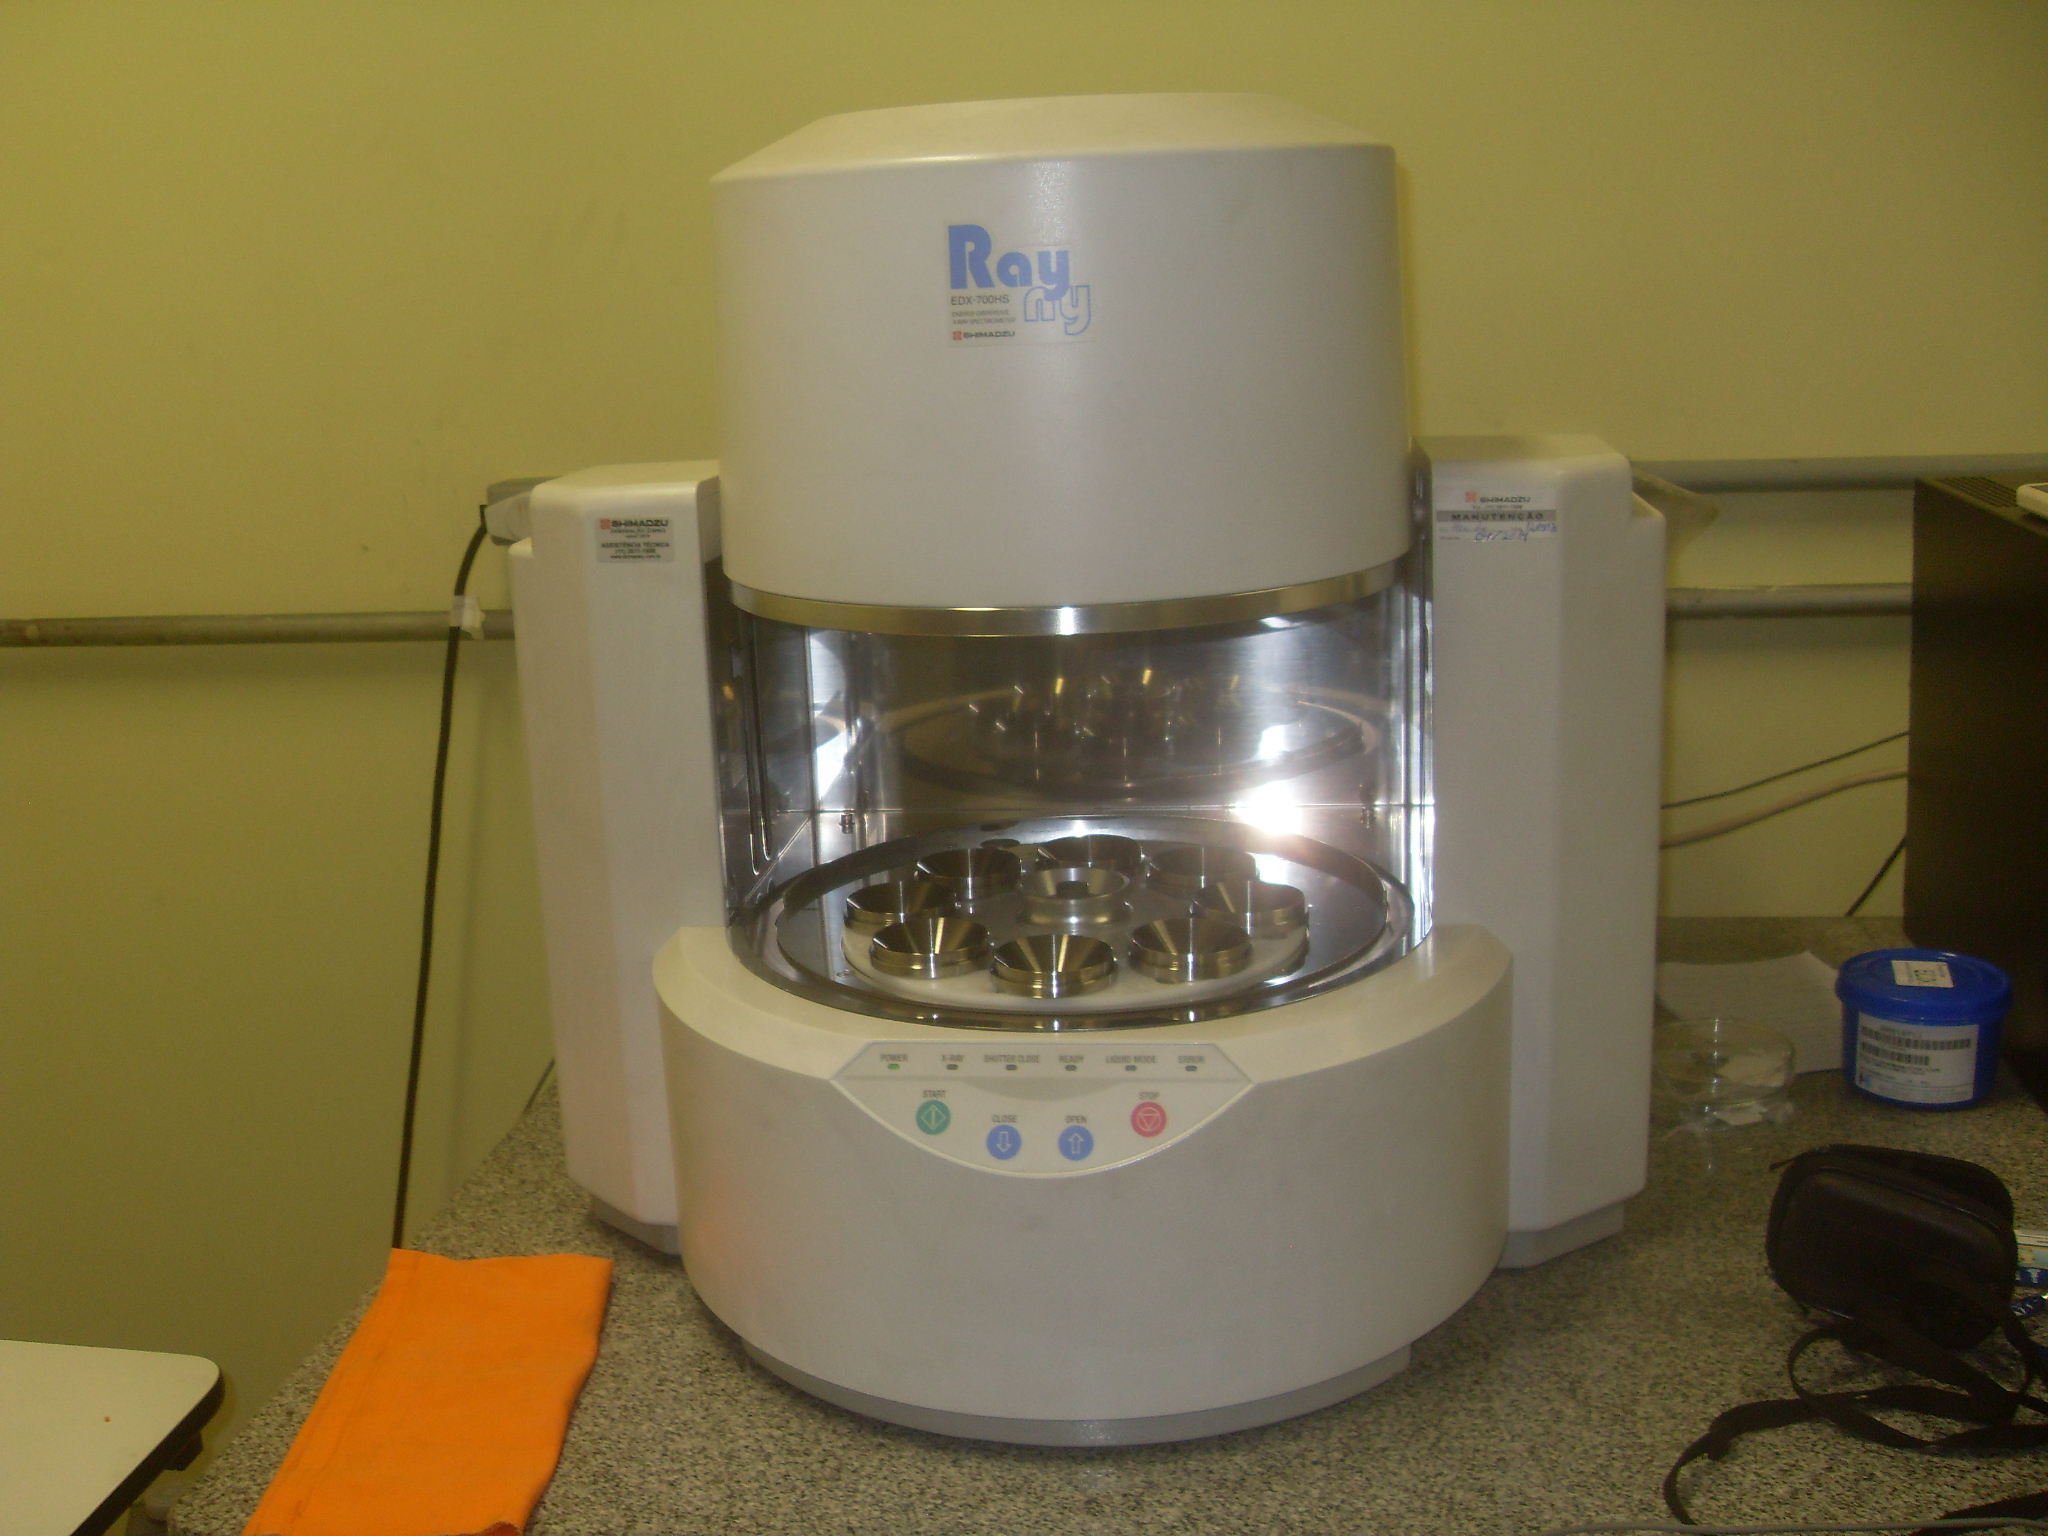
\includegraphics[width=0.5\textwidth]{../inputs/images/xrf-ed-IAG-USP.jpg}
  \caption{XRF-ED Shimadzu modelo EDX 720HS - LAPAt. \label{fig:xrfed_iag}}
\end{figure}

Um tubo de ródio (Rh) submetido a uma diferença de potencial 
de 50 kV foi utilizado para geração do feixe de raios X.
O detector de silício ativado com lítio Si(Li) possui sensibilidade
para medida de fótons com energia entre 1 e 20 keV acoplado a um sistema 
eletrônico com multicanal de 2048 canais capaz de quantificar simultaneamente 
os elementos desde o Na até o Pb. Para remoção da radiação da linha L do feixe 
de raios X do tubo de ródio, de energia próxima de 2,6 keV, um filtro de 
alumínio foi posto entre o feixe e a amostra, melhorando o limite de detecção 
dos elementos com energia igual ou menor que 2,6 keV. O diâmetro do feixe de 
raios X é definido por um colimador de 10 mm, garantindo a irradiação de uma 
área representativa e homogênea da amostra. 

O tempo vivo de irradiação de cada amostra foi $\pm$ 960 minutos, ajustando-se 
a corrente para manter o tempo morto em 20\%. Desejava-se desta forma fixar a 
taxa de contagem, obtendo-se ao final o mesmo número total de fótons contados 
em cada espectro. Esse mecanismo permite melhorar o LD dos elementos presentes 
em amostras menos carregadas. Isso nem sempre foi possível já que a corrente 
máxima no tubo gerador de raios X era de 1000 $\mu A$. 

A figura \ref{fig:xrfed_software} foi extraída do software que acompanha o 
equipamento da Shimadzu e permite verificar em tempo real características
da análise como a voltagem e corrente no tubo, presença e tipo de filtro, 
informação sobre o vácuo na câmera, dentre outros dados que ajudam no 
acompanhamento da análise. 

\begin{figure}[H]
  \centering
  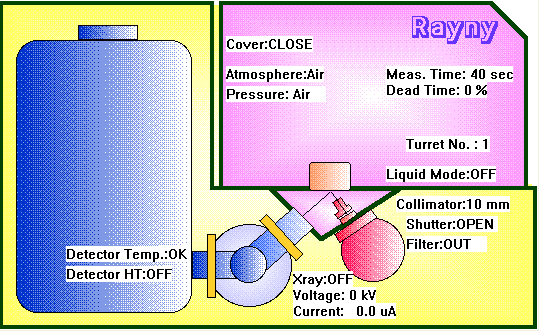
\includegraphics[scale=0.4]{../inputs/images/edx_iag_monitor.png}
  \caption{Software da XRF-ED Shimadzu 720HS, tela de verificação 
           do estado do equipamento. \label{fig:xrfed_software}}
\end{figure}

O EDX 720HS permite análise automática de amostras encaixadas em carrosséis 
de 8 ou 16 posições. O LAPAt contava então apenas com o carrossel de 16 
posições. Foi necessário adquirir um com 8 posições, cujos receptáculos admitiam
o maior diâmetro dos filtros de PTFE, que não podem ser cortados e remontados 
como os de policarbonatos (figura \ref{fig:carrossel8}).

\begin{figure}[H]
  \centering
  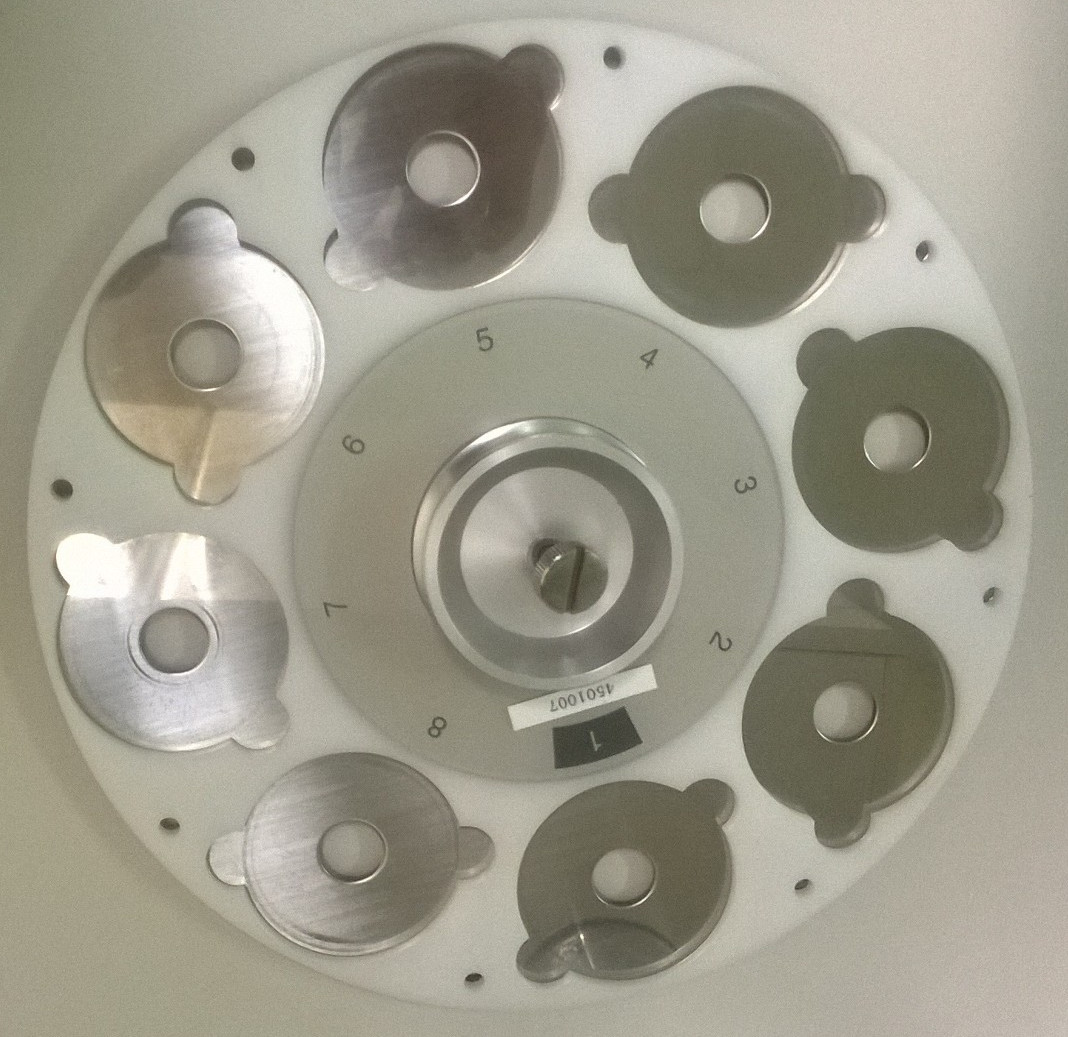
\includegraphics[width=0.5\textwidth]{../inputs/images/carrossel8.jpg}
  \caption{Carrossel de 8 posições adquirido para XRF-ED Shimadzu 720HS. 
           \label{fig:carrossel8}}
\end{figure}

Para eliminar as ondulações típicas que ocorrem nos filtros de PTFE, 
projetou-se um suporte de aço inox que comprimia sua moldura, mantendo plana 
a superfície a ser analisada. Ao mesmo tempo, o peso deste suporte impedia que 
o filtro voasse quando era feito ou quebrado o vácuo na câmera 
(figura \ref{fig:suporte8}).

\begin{figure}[H]
  \centering
  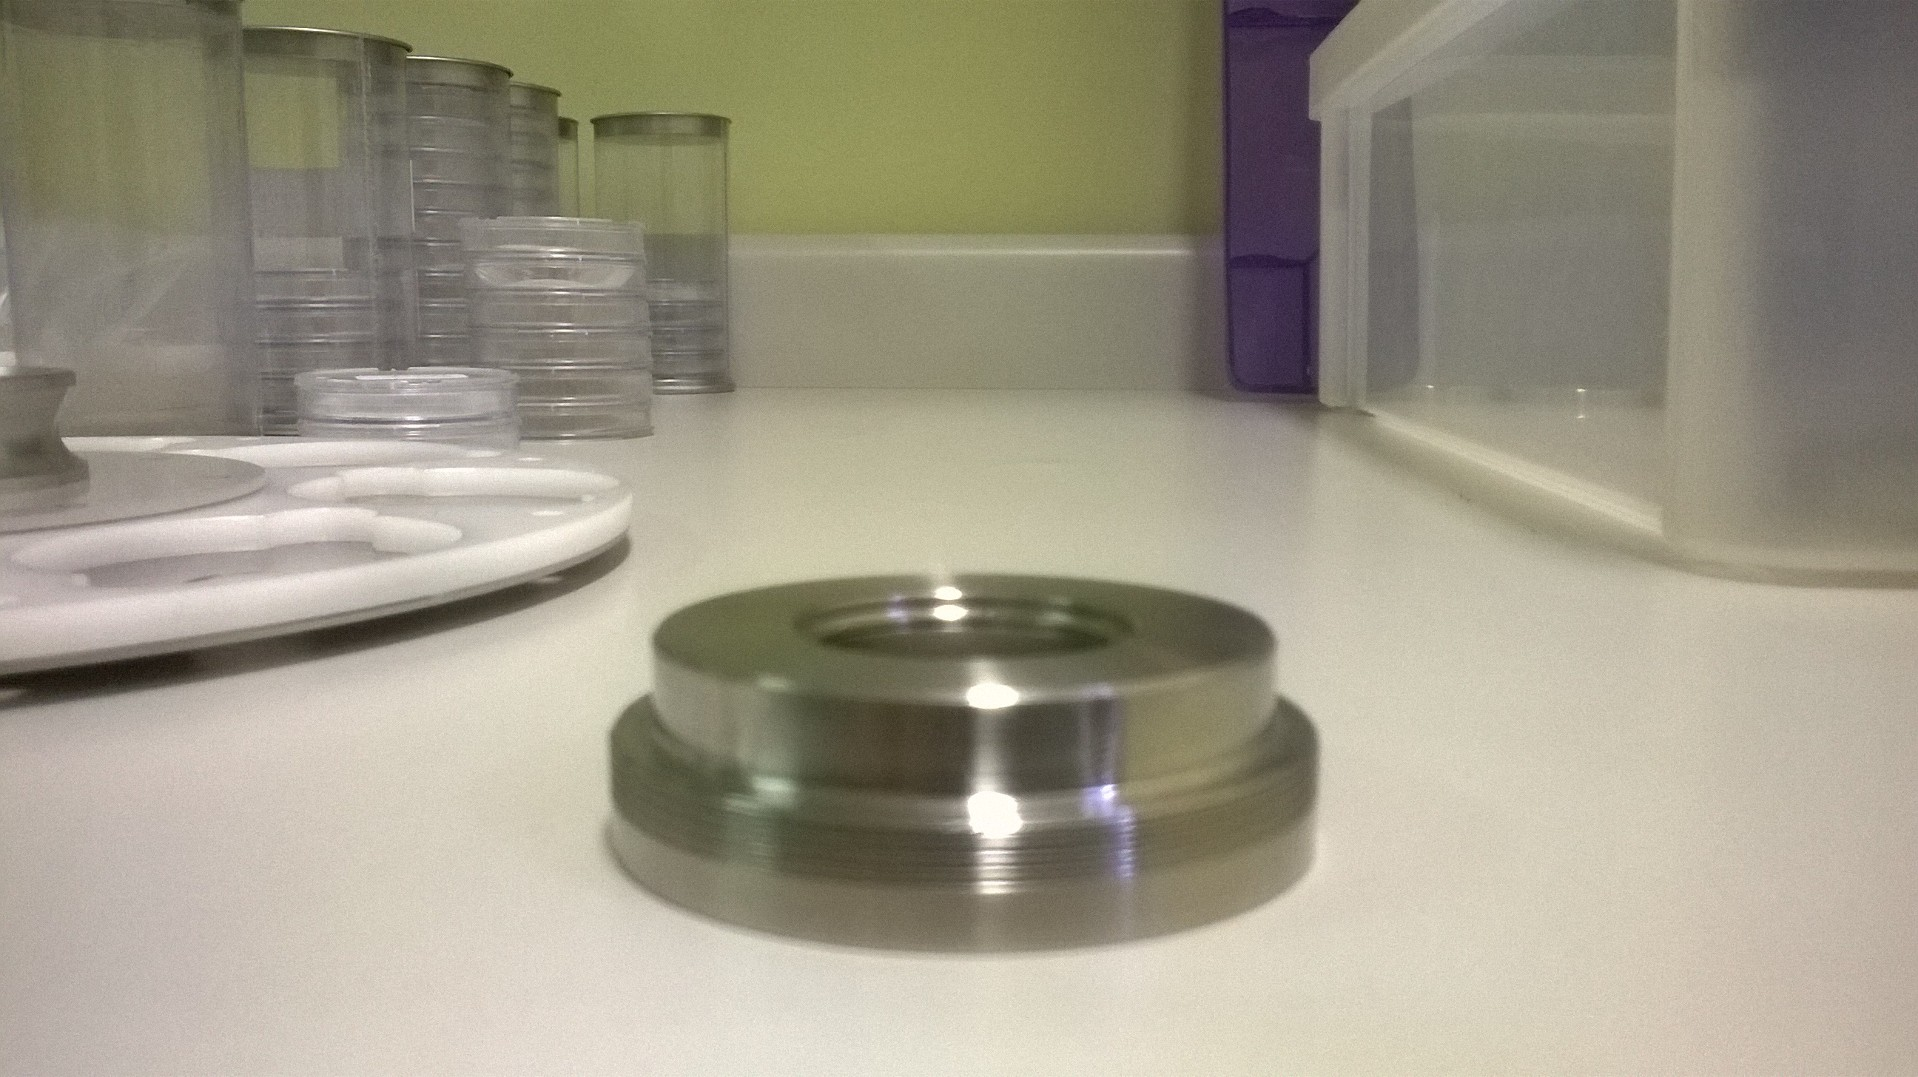
\includegraphics[width=0.5\textwidth]{../inputs/images/suporte8.jpg}
  \caption{Suporte para filtros de PTFE, projetado no LAPAt para carrossel de 
           8 posições e produzido pela oficina da FAP no 
           Instituto de Física da USP. \label{fig:suporte8}}
\end{figure}

%%%%
\subsection{Calibração do XRF-ED}

A massa por unidade de área, depositada sobre os filtros tipicamente usados em 
pesquisas de aerossol atmosférico, permite tratá-los como amostras finas,
ou seja, o efeito de matriz, interações dos raios X característicos com os 
elementos das amostras causando absorção ou reforço do número de fótons de 
raios X característicos, são pequenos diante da precisão do método,
podendo desconsiderá-lo. Nesta aproximação, pode-se relacionar de modo 
simples o número de fótons contados sob o pico característico de um elemento, 
presente no espectro obtido, com a sua massa na amostra irradiada:

\begin{equation}
  \label{eq:contagem}
  N(Z) = R(Z) \cdot I \cdot \Delta t  \cdot \frac{m(Z)}{A}
\end{equation}

Onde R(Z) é chamado de fator de resposta, I é a corrente de excitação do tubo 
de raios X, determinando, portanto, o fluxo de raios X que chegam à amostra, 
$\Delta t$ é o tempo vivo de irradiação e m(Z)/A é a densidade superficial
(massa por unidade de área) dos elementos Z presentes na amostra. 
Pressupõe-se distribuição uniforme da massa na superfície do filtro.

O termo R(Z) depende da seção de choque de cada elemento com o feixe de 
raios X incidente (incluindo modificações por eventuais filtros moduladores 
de suas características), da curva de eficiência do detector de raios X, 
da eficiência de operação do tubo de raios X e da geometria do sistema, 
incluindo os diâmetros de colimadores selecionados. Mantendo estes parâmetros 
fixos e irradiando alvos padrões com densidades (d(Z) = m(Z)/A) 
conhecidas, pode-se calcular R(Z):

\begin{equation}
  \label{eq:fator_de_resposta}
  R(Z) = \frac{N(Z)}{d(Z) \cdot I \Delta t}
\end{equation}

Considerando que a incerteza da corrente e do tempo vivo são desprezíveis 
perto da incerteza da densidade e da contagem, a incerteza no fator de resposta
pode ser calculada por propagação de erro destas variáveis:

\begin{equation}
  \label{eq:erro_fator_de_resposta}
  \sigma_{R(Z)}^2 = {R(Z)}^2 \cdot \left( \left(\frac{\sigma_{N(Z)}}{N(Z)}\right)^2 + 
                                      \left(\frac{\sigma_{d(Z)}}{d(Z)}\right)^2 
                                   \right)
\end{equation}

Dados ambientais são reportados em medidas de concentração ($\mu g/m^3$),
razão da massa m(Z) pelo volume amostrado. Conhecendo o fator de resposta 
R(Z) pode-se calcular a massa m(Z) depositada na amostra, usando a equação 
\ref{eq:contagem}, tomando como valor da área A aquela da deposição de aerossol
no filtro:

\begin{equation}
  \label{eq:xrfedmassa}
  m(Z) = \frac{N(Z) \cdot A}{ R(Z) \cdot I \cdot \Delta t}
\end{equation}

Empregando novamente a expressão da propagação de erro para variáveis 
independentes, a incerteza na massa será:

\begin{equation}
  \label{eq:erro_massa}
  \sigma_{m(Z)}^2 = {m(Z)}^2 \left( \left(\frac{\sigma_{N(Z)}}{N(Z)}\right)^2 + 
                                  \left(\frac{\sigma_A}{A}\right)^2 + 
                                  \left(\frac{\sigma_{R(Z)}}{R(Z)}\right)^2 
                             \right)
\end{equation}


Vê-se, entretanto, que para cada espécie química de interesse, seria necessário
ao menos um alvo de calibração para calcular seu R(Z). Alvos padrões finos, 
com densidade elementar conhecida, podem ser comprados ou produzidos, dependendo
da precisão desejada. Neste projeto foram adquiridos alvos padrões da 
Micromatter, com incerteza nominal de 5\%. Mas esta empresa não produz alvos 
com proporção estequiométrica quantificada para todas espécies químicas.
Assim, trouxemos para a XRF-ED o conceito proposto por \citet{tabacniks2000}
implementado no sistema PIXE (Particle Induced X-Ray Emission) do IFUSP que permite obter uma 
calibração abrangendo elementos de número atômico no intervalo 10 < Z < 83. 
 
Adotou-se, ainda, uma metodologia estatística robusta para estimativa das 
incertezas da calibração usando MQM. Essa preocupação em definir 
adequadamente as incertezas deve-se, particularmente, ao fato de que elas 
ponderam o peso das variáveis na modelagem por PMF.

Como exemplo para conhecer o forma da curva de calibração, o gráfico da figura 
\ref{fg:edxrfcalib} apresenta os R(Z) dos alvos padrões da Micromatter 
irradiados em maio de 2010. 

\begin{figure}[H]
  \begin{subfigure}[b]{0.45\textwidth}
    \includegraphics[width=\textwidth]{../outputs/plot_R_maio2010K.pdf}
    \caption{linha K}
  \end{subfigure}%
  \begin{subfigure}[b]{0.45\textwidth}
    \includegraphics[width=\textwidth]{../outputs/plot_R_maio2010L.pdf}
    \caption{linha L}
  \end{subfigure}
  \caption{Fatores de respostas, R(Z), para alvos padrões da 
           Micromatter irradiados em maio de 2010. 
           \label{fg:edxrfcalib}}
\end{figure}

Nota-se que é possível fazer um ajuste polinomial sobre esses dados, 
o que tanto melhora a precisão para todos os R(Z), quanto fornece seu valor
para elementos que não possuem alvos padrões. O fator de resposta reflete 
o arranjo experimental, mudanças físicas
nesse arranjo alteram o valor de R(Z), assim como a progressiva fadiga do detector
ou do tubo. Portanto, a calibração deve ser realizada periodicamente.

%%%%
\subsection{Incertezas dos ajustes com Mínimos Quadrados Matricial}

As incertezas dos ajustes polinomiais das calibrações do XRF-ED e da 
intercalibração de TOT e refletância de BC foram estimadas com o método 
Mínimos Quadrados Matricial (MQM) desenvolvida por \citet{helene2006}
e parcialmente reproduzida a seguir (com adaptações).

Dadas as variáveis $Y_i$ e $X_i$ relacionadas polinomialmente:

\begin{equation}
  \label{eq:polinomio}
  \begin{split}
    y_1 = a + b x_1 + c{x_1}^2 + d{x_1}^3 + ...\\
    y_2 = a + b x_2 + c{x_2}^2 + d{x_2}^3 + ... \\
    ...
  \end{split}
\end{equation}

ou na forma matricial:

\begin{equation}
  \label{eq:polinomioMatriz}
  [Y] = [A][X]
\end{equation}

Os coeficientes ajustados [Ã] são dados por:

\begin{equation}
  \label{eq:coeficientesajustados}
  [Ã] = [V_{Ã}] ([X]^T {[V_Y]}^{-1} [Y])
\end{equation}

Sendo $[V_{Ã}]$ a matriz de covariância dos coeficientes, dada por:

\begin{equation}
  \label{eq:matrizcovariancia}
  [V_{Ã}] = ([X]^T [V_Y]^{-1} [X])^{-1}
\end{equation}

A partir dos coeficientes ajustados [Ã] na equação \ref{eq:coeficientesajustados},
pode-se calcular os $[\tilde{Y}]$ ajustados,

\begin{equation}
  \label{eq:polinomioajustado}
  [\tilde{Y}] = [Ã][X]
\end{equation}

A diagonal da matriz de covariância de $[\tilde{Y}]$, $[V_{\tilde{Y}}]$, 
representa a incerteza dos valores ajustados:

\begin{equation}
  \label{eq:matrizcovarianciaY}
  [V_{\tilde{Y}}] = [X] [V_{Ã}]^{-1} [X]^{-1}
\end{equation}

No caso da XRF-ED, quando se calcula R(Z) apenas a partir do alvo de 
calibração do elemento Z, é a incerteza de produção deste alvo que determina 
a precisão de R(Z). Mas com o procedimento de ajuste por MQM, sob os 
R(Z) disponíveis, é o conjunto destes valores e de suas incertezas, bem como a 
qualidade do ajuste que determinam a incerteza ajustada, oferecendo uma 
melhora significativa na precisão e na exatidão dos R(Z).

%%%%
\subsection{Fontes de erro no branco}

A massa depositada no filtro amostrado $m(Z)_{medido}$ para um certo elemento Z
é composta pela massa coletada na amostragem m(Z) mais a massa do filtro 
branco $m_{B}(Z)$.

Um conjunto de 10 amostras brancas (entre campo e laboratório) foram analisadas, 
para eliminação da contaminação dos próprios filtros, assim como de 
transporte e manipulação.

A seguir, a equação \ref{eq:contagem} está escrita para representar o número de contagens de alvos amostrados, isto é, com sobreposição da massa coletada na amostragem $m(Z)$ e a massa do branco $m_B(Z)$: 

\begin{equation}
  \label{eq:contagem_medida}
  N(Z)_{medido} = R(Z) \cdot I \cdot \Delta t \cdot \left( \frac{m(Z)}{A} + \frac{m_B(Z)}{A} \right)
\end{equation}  

Quando as amostras brancas são irradiadas separadamente, o número de contagens é dado por:

\begin{equation}
  \label{eq:contagembranco}
  N_B(Z) = R(Z) \cdot I_B \cdot \Delta t_B \cdot \frac{m_B(Z)}{A}
\end{equation}

Isolando-se $m_B(Z)$ em \ref{eq:contagembranco} e substituindo em 
\ref{eq:contagem_medida}, encontramos o número de contagens corrigido nos alvos amostrados
(isto é, excluindo a contaminação das amostras brancas):
 
\begin{equation}
  \label{eq:contagemcorrigida}
  N(Z) = N(Z)_{medido} - I \cdot \Delta t \cdot \left( \frac{N_B}{I_B \cdot \Delta t_B}  \right)
\end{equation}

A incerteza da contagem corrigida (equação \ref{eq:contagemcorrigida}) é dada por:

\begin{equation}
  \label{eq:erro_contagemcorrigida}
  \sigma_{N(Z)}^2 = \sigma_{N(Z)_{medido}}^2 + \left( \frac{I \cdot \Delta t}{I_B \cdot \Delta t_B} \right)^2 \cdot \sigma_{N_B}^2
\end{equation}

Calcula-se a razão $N_B/(I_B \cdot \Delta t_B)$ para um conjunto de alvos brancos para 
posterior inserção na equação \ref{eq:contagemcorrigida}.

Foi criado colaborativamente por pesquisadores do LAPAt um programa 
em linguagem C que automatiza o cálculo teórico de concentrações apresentado, 
com as devidas correções de branco e propagações de incertezas \footnote{
O código está disponível no repositório de versionamento git da USP 
e pode ser acessado pelo endereço: 
\url{https://git.uspdigital.usp.br/5385361/xrfdensid}}.

%%%%
\subsection{Integração dos espectros}

Realizou-se a integração de todos os espectros obtidos na XRF-ED no
Quantitative X-Ray Analysis System for Windows (WinQxas),
programa desenvolvido para integração numérica de espectros sob o patrocínio 
da Agência Internacional de Energia Atômica (IAEA) \citep{capote2000}.

Obtém-se os parâmetros iniciais da relação linear entre canal e energia,
conhecendo-se ao menos dois picos no espectro, normalmente Ferro e Cálcio, 
no caso de poluição do ar ambiental. 

Os parâmetros iniciais entre a largura do pico à meia altura (FWHM)
dependem da energia (E), do nível geral de ruído (NOISE) no espectro 
e do FANO, dado pela relação: 

\begin{equation}
  \label{eq:fwhm}
   {FWHM}^2 = {NOISE}^2 + 2,35 \cdot FANO  \cdot E
\end{equation}

Os parâmetros iniciais foram determinados a partir de espectros com picos 
bem definidos, como o Ferro, que teve largura à meia altura (FWHM) para 
$K\alpha$ de 138,32 eV ou o Cálcio com 129,14 eV.

Na figura \ref{fig:winqxas} há dois exemplos de espectros abertos no WinQxas
para amostras de Nima, sendo um de uma amostra branca e a outra carregada. Os picos 
característicos de elementos químicos encontrados estão indicados na figura.

\begin{figure}[H]
  \centering
  \begin{subfigure}[b]{0.7\textwidth}
    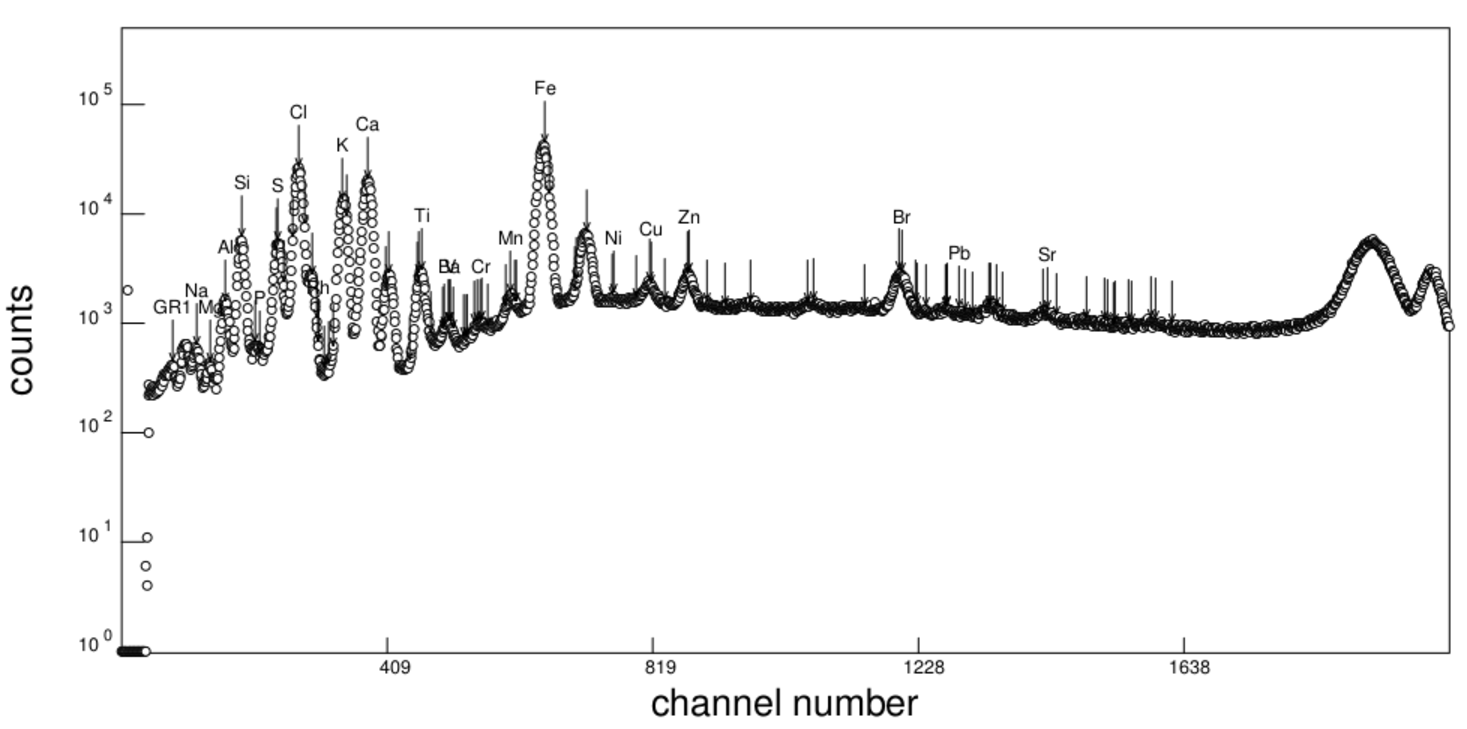
\includegraphics[width=\textwidth]{../inputs/images/winqxas/GHA41editado.pdf}
    \caption{Espectro de amostra carregada (GHA41) - Acra Nima}
  \end{subfigure}
  \begin{subfigure}[b]{0.7\textwidth}
    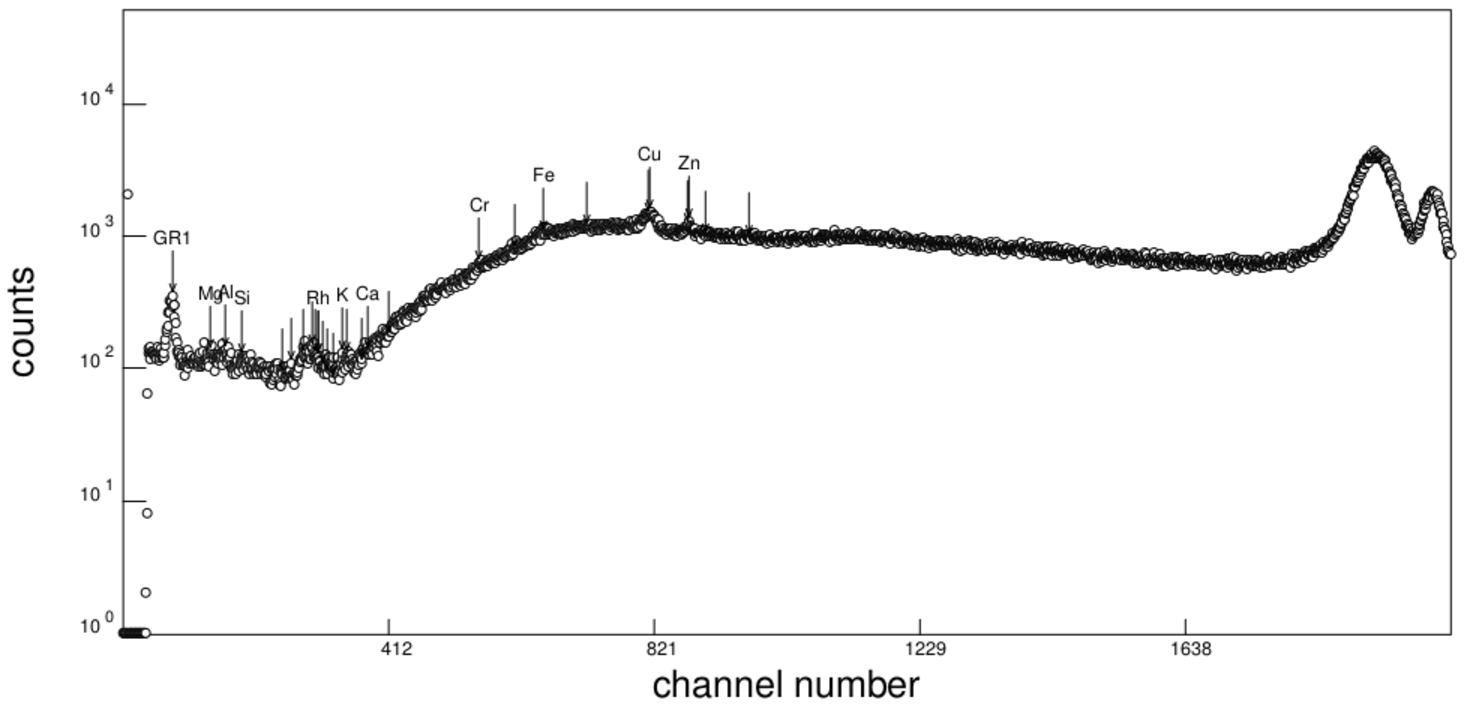
\includegraphics[width=\textwidth]{../inputs/images/winqxas/GPE770editado.pdf}
     \caption{Espectro de amostra branca (GPE770)- Acra Nima}
  \end{subfigure}
  \caption{Espectros para amostra branca e carregada de Nima. \label{fig:winqxas}}
\end{figure}

Na integração dos espectros, pico a pico, deve-se ter atenção 
para identificação e correção dos seguintes eventos em picos com 
muitas contagens: 

\begin{itemize}
  \begin{spacing}{1.0}
  \item pico soma: quando fótons de diferentes elementos são contados
        juntos pelo detector. 
  \item pico escape: quando o fóton incidente excita o silício do detector
        e é contado com energia menor, pois parte foi perdida na excitação 
        do silício. 
  \end{spacing}
\end{itemize}

A seguir, apresenta-se a calibração do multicanal, ajuste linear entre canal 
e energia encontrado a partir do Fe e Ca:

\begin{equation}
  E = 0,0101 \cdot Canal - 0,1335 (keV)
\end{equation}

%%%%
\subsection{Limite de detecção}

O limite de detecção (LD) é a intensidade mínima do pico de um elemento para haver 
detecção da espécie se considerando o tipo de filtro e XRF-ED empregados. 
Irradiando uma amostra branca, obtém-se o número de contagens 
medidas ($N_{fundo}$) sob o pico (fundo do espectro) de cada um dos elementos
medidos.
As contagens de fundo do espectro seguem uma distribuição de Poisson e portanto 
a incerteza para o valor de N contagens é $\sqrt{N}$.
Desta forma, adota-se como LD para um elemento, a condição de que as contagens de seu pico 
característico seja pelo menos três vezes a incerteza na contagem de fundo:

\begin{equation}
  \label{eq:limitedeteccao}
  N_{LD} = 3 \cdot \sqrt{N_{fundo}}
\end{equation}

Pode-se calcular o LD em termos da massa elementar com a 
equação \ref{eq:xrfedmassa}. O limite de detecção muda conforme a quantidade de 
material coletado, sendo maior em amostras carregadas, devido à sobreposição de 
picos e a maior reflexão do feixe na amostra.

Assim, o ideal é calcular o LD em cada amostra, mas ele deve situar-se entre 
aquele medido em um filtro branco e uma amostra com bastante carga.
Os LDs encontrados para os dois tipos de amostras estão apresentados 
nos gráficos da figura \ref{table:ld} em termos de concentrações típicas 
($\mu g / m^3$) para o volume médio de 13,9 $m^3$. 
Note-se que na linha K o LD é alto para elementos de baixo número atômico, 
dificultando a detecção desses elementos, mas melhora com o aumento de Z. 

\begin{figure}[H]
  \begin{subfigure}[b]{0.5\textwidth}
    \includegraphics[width=\textwidth]{../outputs/limitDetectionK.pdf}
    \caption{linha K}
  \end{subfigure}%
  \begin{subfigure}[b]{0.5\textwidth}
    \includegraphics[width=\textwidth]{../outputs/limitDetectionL.pdf}
    \caption{linha L}
  \end{subfigure}
  \caption{Limite de detecção para XRF-ED em termos de concentrações típicas 
           para amostra branca e carregada.
           \label{table:ld}}
\end{figure}

\newpage
\begin{table}[H]
  \centering
  \input{../outputs/LD.tex}
  \caption{Limite de detecção para XRF-ED em termos de concentrações típicas 
           para amostra branca e carregada. \label{table:LD}}
\end{table}

%%%%
\section{Black Carbon}

Medidas de BC pela técnica de refletância apresentam a vantagem de poderem ser 
realizadas sobre os mesmos filtros empregados para análises gravimétricas, 
XRF ou mesmo em técnicas destrutivas que posteriormente possam vir a ser 
realizadas sobre eles, como cromatografia iônica ou espectroscopia de massa. 
Isso promove a redução das incertezas provenientes de análises que pedem 
diferentes amostradores coletados em paralelo. Também pode diminuir 
significativamente a dimensão da instrumentação em uma pesquisa. Entretanto, 
a refletância é uma medida indireta, cujo resultado depende das características 
do aerossol amostrado. Utilizando o método absoluto TOT para algumas amostras, 
foi possível intercalibrar as medidas de refletância com esse método absoluto, 
permitindo a quantificação do BC nas demais amostras.

%%%%
\subsection{Calibração da refletância usando BC Monarch 71}

Alvos padrões produzidos no laboratório do antigo GEPA-IFUSP (Grupo de Estudos 
de Poluição do Ar), hoje Laboratório de Física Atmosférica (LFA-IFUSP), 
com concentrações conhecidas do BC de referência Monarch 71 (M71) 
\citep{clarke1986}, foram usados por décadas em equipamentos de refletância 
alocados nestes laboratórios e no LAPAt, para a calibração de refletância versus
densidade superficial de BC em filtros que coletaram aerossol atmosférico.

A tabela \ref{table:monarch71} mostra um conjunto de valores medidos em 2007 
para estes padrões (com respectivas médias e incertezas), sobre os quais foi 
feita uma calibração no Lapat, seguindo exatamente os mesmos procedimentos do 
GEPA/LFA-IFUSP. Os novos parâmetros então ajustados ofereciam resultados 
apenas 2,3\% menores que a calibração anterior (1994), do GEPA/LFA-IFUSP. 
Isso revela equipamentos uniformes e grande estabilidade destes padrões. 
Entretanto, essa sistemática de calibração padecia de três problemas.

O primeiro deles refere-se à estreita faixa de valores oferecidas por estes 
padrões que, como pode ser visto na referida tabela, variam entre 30\% e 85\%, 
não cobrindo a região acima de 85\% ou abaixo de 30\%, esta última onde 
posicionam-se os filtros carregados que encontramos no experimento de Gana. 
Mesmo assim, se fosse considerada a linearidade que predomina na relação 
entre densidade de BC e log da refletância, equação \ref{m/a_2}, e acrescida 
no ajuste a massa zero, para qual a refletância é 100\% ($log_{10}$100 = 2), 
poder-se-ia estender o ajuste para uma faixa apreciável de valores.
Mas a função adotada para os ajustes foi uma parábola. Esse foi um segundo 
problema para esta calibração, como se pode verificar na figura 
\ref{fig:monarch71}, essa função distancia-se bastante de um ajuste linear 
conforme nos deslocamos em direção a $log_{10}$ 10, ponto em que a relação da 
massa com o log da refletância começa a perder a linearidade. O gráfico da 
figura \ref{fig:razaoTOTM71} mostra que a margem de erro em alvos carregados 
cresce com o ajuste de 2$\degree$ grau, quando confrontado com a calibração 
baseada em TOT, para filtros coletados em Gana. Note-se, entretanto, que na 
zona de refletância onde havia alvos padrões, as diferenças com o método 
absoluto, por óbvio, são semelhantes. 

A calibração do refletômetro do LAPAt para 2007 usando alvos padrões M71 com 
ajuste de primeiro grau está no gráfico da figura \ref{fig:monarch71}, com 
respectivos dados apresentados na tabela \ref{table:monarch71}.

\begin{figure}[H]
  \centering
  \includegraphics[width=0.5\textwidth]{../outputs/BC_monarch71.pdf}
  \caption{Calibração do refletômetro do LAPAt em 2007 usando alvos padrões M71.
         \label{fig:monarch71}}
\end{figure}

\newpage
\begin{table}[H]
  \centering
  \small
    \input{../outputs/BC_monarch71.tex}
    \caption{Calibração do refletômetro do LAPAt em 2007 usando alvos padrões 
             M71. \label{table:monarch71}}
\end{table}

Procuramos construir uma calibração mais consistente, produzindo alvos de 
calibração que cobrissem toda a faixa de valores entre 0 a 100\% de refletância. 
Mas não encontramos mais o BC M71 para comercializar, assim usamos o BC de 
referência (ASTM-N762) do IPT com o qual produzimos 27 padrões depositados em 
filtros de policarbonato (nuclepore fino de 37 mm, orifícios de 0,4 $\mu m$) 
usando amostrador dicotômico (diâmetro de corte em 2,5 $\mu m$) na câmara de 
ressuspensão do laboratórios da Divisão de Qualidade do Ar da CETESB.

Os valores de refletância nesses filtros variaram de 3,1\% até 98,7\%, mais um 
"zero" de massa teórico com refletância 100\%. As massas foram medidas em 
microbalança analítica $\pm$ 1 g. A figura \ref{fig:bc_cetesb} mostra o ajuste 
entre massa de BC depositada versus o log da refletância medida. Pode-se ver 
que o ajuste linear foi excelente,
indicando que a calibração deve perder linearidade apenas em refletâncias 
inferiores a 5\%.

\newpage
\begin{table}[H]
	\centering
	\small
	\input{../outputs/cetesb2012.tex}
	\caption{Reflêtancia de filtros produzidos na cetesb. \label{table:bc_cetesb}}
\end{table} 

\begin{figure}[H]
	\centering
	\includegraphics[width=0.5\linewidth]{../outputs/BC_cetesb.pdf}
	\caption{Reflêtancia de filtros produzidos na cetesb. \label{fig:bc_cetesb}}
\end{figure}

As barras de erros nas massas correspondem ao erro efetivo $\sigma_{efetivo}$, 
o qual é a adição (soma dos quadrados) do erro propagado da refletância (eixo x)
com o erro de medida da massa (eixo y). Como a relação entre x e y é linear, 
a incerteza em y devido a x pode ser escrita como:

\begin{equation}
  {\sigma_y}_x = \frac{\partial y}{\partial x} \cdot \sigma_x
\end{equation} 

Usada na soma dos quadrados para calcular a incerteza efetiva em y, 
$\sigma_{efetiva}$: 

\begin{equation}
  \sigma_{efetiva} = \sqrt{{\sigma_y}^2 + {{\sigma_y}_x}^2}
\end{equation} 

Como a menor medida na leitura do aparelho digital de refletância é 0,1\%
(o \% aqui é a unidade de medida para refletância) é muito baixa, estimamos 
a incerteza na refletância a partir da oscilação na alvura do substrato de 
amostragem calculando o desvio padrão para sete amostras 
brancas ($\sigma$=0,957 \%). Aplicamos correção de fator 1,11 devido ao 
espaço amostral pequeno \citep{helene1981}, resultando em $\sigma$=1,06 \%.

Infelizmente, como veremos a seguir, no confronto com TOT, o BC utilizado 
mostrou ter características bastante diversas do BC encontrado regularmente 
na atmosfera, introduzindo um erro sistemático da ordem de um fator 5.  


%%%%
\newpage
\subsection{Calibração com TOT - Experiência nos túneis Jânio Quadros e Rodoanel}

Em maio de 2011, simultaneamente ao período de análises das amostras de Gana, 
conduzia-se experimento para analisar as emissões veiculares na cidade de São 
Paulo. As medidas foram feitas no interior dos túneis Jânio Quadros e Rodoanel,
que têm características de circulação predominante de veículos leves e pesados 
(ou diesel), respectivamente. 

Tomou-se amostragens simultâneas de $MP_{2,5}$, por amostrador MiniVol com 
filtros de quartzo e por amostrador Partisol com filtros de policarbonato, 
sendo o primeiro para medida absoluta de EC por TOT e o segundo para análises
de XRF-ED, medida relativa de BC por refletância e para cromatografia iônica.

Tamanha era a poluição dos caminhões que os filtros coletados no Rodoanel 
ficaram saturados para medidas de BC por refletância (valores próximos a zero), 
o que impossibilitou usá-los para fins de calibração. No túnel Jânio Quadros as 
refletâncias variaram de 4,9 a 57,1\%, permitindo a calibração da refletância 
por TOT.

A determinação BC por TOT nos filtros de quartzo foi conduzida pelo Dr. Pierre 
Herckes, do Departamento de Química e Bioquímica da Universidade Estadual do 
Arizona. Contou-se com 16 filtros coletados no túnel Jânio Quadros. 
O gráfico da figura \ref{table:interJQ} apresenta a intercalibração com ajuste 
linear entre as medidas de TOT nas amostras dos filtros de quartzo e a 
refletância das 16 amostras correspondentes nos filtros de policarbonato.
Nota-se a boa qualidade do ajuste linear de calibração da densidade superficial 
de massa de BC versus o log da refletância por TOT no túnel Jânio Quadros. 

\begin{figure}[H]
  \centering
  \includegraphics[width=0.5\linewidth]{../outputs/JQ_TOT_Refletancia.pdf}
  \caption{Intercalibração TOT e Reflêtancia para amostragem paralela no 
           túnel Jânio Quadros. \label{table:interJQ}}
\end{figure}

Buscou-se, também, confrontar a massa obtida pela calibração com os  
alvos de BC comercial elaborados no laboratório da CETESB, com a massa 
obtida pela calibração via TOT, gráfico da figura \ref{fig:JQ} e tabela
\ref{table:JQ}. Apesar da excelente relação linear de ambas calibrações, os 
valores de massa calculados diferiram em aproximadamente um fator 5, sendo as 
massas calculadas com a calibração da CETESB maiores que a por TOT.  
Como já mencionamos, isso significa que o BC comercial (ASTM-N762) tem 
propriedades diferentes daquele BC que compõe o aerossol coletado no túnel do 
Jânio Quadros, provavelmente, sua granulometria seria mais grossa, o que gera 
menos superfície de absorção por muito mais massa coletada. Neste sentido, ele 
não seria indicado para calibrações realistas de equipamentos de refletância. 

\begin{figure}[H]
  \centering
  \begin{minipage}[b]{0.5\linewidth}
    \includegraphics[width=\textwidth]{../outputs/BC_janio_quadros.pdf}
    \caption{Comparação da massa de BC das amostras do túnel Jânio Quadros 
             calculada usando calibração por TOT versus calibração a partir dos 
             alvos padrões produzidos na CETESB. \label{fig:JQ}}
  \end{minipage}
  \hspace{0.5cm}
  \begin{minipage}[b]{0.45\linewidth}
    \begin{small}
      \input{../outputs/BC_janio_quadros.tex}
    \end{small}
    \captionof{table}{Comparação da massa de BC das amostras do túnel Jânio Quadros 
             calculada usando calibração por TOT(1) versus calibração a partir dos 
             alvos padrões produzidos na CETESB(2). \label{table:JQ}}
  \end{minipage}
\end{figure}

\newpage
%%%%
\subsection{Intercalibração de TOT e refletância para Acra}

Como discutido na descrição da metodologia analítica para BC, as características
de tamanho, forma geométrica e seção de choque de absorção de luz das 
partículas de BC variam de região para região.
Por esses motivos, é importante fazer a comparação de método indireto com método
direto \citep{quincey2007}. \citet{taha2007} também aponta que há uma limitação 
da técnica de refletância quando filtros de teflon são usados, pois em altas 
concentrações (refletâncias inferiores a 20\%), ocorre saturação, e a 
relação exponencial da equação \ref{m/a_2} passa a não valer 
mais. 

Dos 2898 filtros PTFE coletados no experimento de Gana, 52 tiveram medidas 
paralelas em filtros de quartzo para $MP_{2,5}$, analisados por TOT.
Os filtros coletados em Acra apresentaram refletância pequena, pois além da 
alta poluição atmosférica o tempo de amostragem de 48 horas contribuiu para que
as amostras ficassem muito carregadas. Buscou-se então proceder como no 
experimento do túnel Jânio Quadros em São Paulo, intercalibrando a refletância 
com as medidas de TOT disponíveis, de forma a estimar os valores de BC em todos 
filtros PTFE de $MP_{2,5}$. O gráfico da figura \ref{fig:interGanaBC} e a 
tabela \label{table:interGanaBC} mostram o ajuste realizado, já contabilizando 
um ponto de massa zero no ajuste. A incerteza efetiva considera o erro do TOT 
e da refletância, além dos 8\% de amostragem paralela. 

Assumimos como incerteza para os valores de refletância (medido em porcentagem)
o desvio padrão corrigido das medições de 7 filtros em branco 
(média = 0,96\% x 1,11 = 1,06\%), corrigidos para as estatísticas de poucos 
dados, utilizando 7 valores). A incerteza em massa acumulada foi de $sqrt(2)$.

O gráfico da figura \ref{fig:razaoTOTM71} mostra a relação entre a calibração do 
BC por TOT e o resultado que teríamos se empregássemos a calibração 
tradicionalmente feita com M71. Neste último caso o ajuste foi feito com uma
reta, como diz a relação derivada para absorção, e uma curva parabólica, 
como usualmente empregada no laboratório. Na região onde existem alvos padrões, 
os ajustes de primeiro e segundo grau apresentam concordância com os valores 
obtidos por TOT, mas em altas concentrações, o ajuste linear proveria resultados
mais próximos daqueles obtidos por calibração TOT, mesmo assim com diferenças 
em torno de 25\%. 

Fazendo-se a mesma comparação para filtros analisados em Recife \citep{santos2014},
as diferenças oscilavam entre um fator 1,4 e 2,4 (figura \ref{fig:BC_compara_recife}).

O uso de refletância mostrou-se bastante eficiente para determinação de BC, 
sendo aconselhável, entretanto, prover a calibração de um conjunto de filtros 
com um sistema de medida absoluto como o TOT.


\begin{figure}[H]
	\begin{center}
		\includegraphics[width=0.9\textwidth]{../outputs/Gana_TOT_Refletancia.pdf}
		\caption{Intercalibração entre TOT e refletância em Acra. \label{fig:interGanaBC}}
	\end{center}
\end{figure}

\begin{figure}[H]
	\centering
	\begin{subfigure}[b]{0.43\linewidth}
		\includegraphics[width=\linewidth]{../outputs/BC_compara_calibs.pdf}
		\caption{Acra \label{fig:razaoTOTM71}}
	\end{subfigure}
		\hspace{0.3cm}
	\begin{subfigure}[b]{0.43\linewidth}
		\includegraphics[width=\linewidth]{../outputs/BC_compara_calibs_recife.pdf}
		\caption{Recife \label{fig:BC_compara_recife}}
	\end{subfigure}%

	\caption{Razão dos valores de BC medidos por refletância e calibrados por 
		TOT e M71 para Recife e Acra. \label{fig:BC_compara}}
\end{figure}

\begin{table}[H]
	\centering
	\small
	\input{../outputs/Gana_TOT_Refletancia.tex}
	\caption{Intercalibração entre TOT e refletância em Acra. \label{table:interGanaBC}} 
\end{table} 



%%%%
\section{Modelos Receptores}

Modelo receptor é uma abordagem matemática para determinar e 
quantificar o efeito das fontes poluidoras do ar. 

Modelos receptores buscam quantificar a participação de fontes poluidoras em amostras. 
O Balanço Químico de Massas (CBM), por exemplo, necessita do conhecimento prévio do 
perfil das fontes locais, cuja combinação linear proverá o rateio de amostragens 
entre tais fontes. 

Já a Análise de Fatores Principais (PFA) ou Positive Matrix Fatorization (PMF)
permitem o rateio de fontes quando os seus perfis são desconhecidos. 
Entretanto, necessitamos de conhecê-los quando buscamos associar estes 
resultados a realidade concreta da bacia aérea estudada. 

%TODO: no site da cetesb tem um esquema legal de modelo receptor
%TODO: traçar um panomara da evolução histórica dos modelos receptores.

\subsection{Análise multivariada}

O processo de identificação das fontes de poluição do ar é 
complexo, havendo diversos caminhos, os quais as técnicas estatísticas
multivariadas são historicamente usadas.
 
Análise multivariada é uma das técnicas estatística utilizadas para 
resolver reduzir a dimensão dos dados coletados nos modelos receptores, 
usando a variância. 

As dimensões (variáveis) reduzidas de um conjunto de dados analíticos 
complexo poderão ser interpretados como fonte(s) poluídora(s).

As técnicas de redução da dimensão, como análise multivariada, 
permitem manter a quantidade de informação contida inicialmente nos dados. 
Essa informação está armazenada na variância e covariância (ou correlação) 
inicial dos dados. 

Dâ-se o nome de Fator as novas variáveis reduzidas. 
O Fator é um tipo de variável latente, pois não é uma grandeza diretamente
medida, mas sim obtida a partir de outras variáveis observáveis. 

O número de fatores extraídos dependerá do conhecimento do(a) pesquisador(a)
sobre a região, possíveis fontes poluidoras, número de amostras, 
resolução da amostragem e espécies medidas.

O conhecimento do pesquisador é imprescindível para fazer o relacionamento 
entre fator e fonte(s), afim de avaliar o significado físico das fontes. 
Para tal, informações das possíveis fontes poluidoras próximas ao ponto 
receptor, dados meteorológicos do período de coleta, inventário de emissões 
e outras informações que possam ajudar a fazer esse relacionamento 
devem ser usadas.

Número reduzido de amostras, baixa resolução da amostragem, \textbf{outliers} 
(eventos infrequentes de curta duração e com alta concentração) representam 
um desafio para modelos multivariados.

%%%%
\subsection{Fomulação matemática dos Modelos Receptores}

Os poluentes que são emitidos pelas fontes em uma bacia aérea devem chegar no 
receptor, podendo-se, assim, usar o princípio de conservação de massa no Modelo Receptor. 
Vamos fazer uma adaptação da equação de conservação de massa para o contexto 
de poluição do ar. 

Se em uma amostragem coletamos $j$ amostras e medimos $i$ poluentes, podemos 
escrever a equação da conservação de massa como segue: 

\begin{equation}
  x_{ij} = \sum_{p=1}^{P} g_{ip}f_{pj} + \epsilon_{ij}
\end{equation} 

sendo,
\begin{itemize}
  \item $x_{ij}$ = concentração na amostra receptora $i$ da espécie $j$;
  \item $f_{pj}$ = fração da espécie $j$ emitida pela fonte $p$;
  \item $g_{ip}$ = contribuição da fonte $p$ para amostra $i$;
  \item $\epsilon$ = erro do modelo empregado.
\end{itemize}

%%%%
\subsection{Balanço Químico de Massa}

O quanto dos perfis de fontes medidas explica as concentrações dos elementos? 
A técnica Balanço Químico de Massa (\textbf{BQM}) busca responder essa questão.

%TODO: você deve terminar de dizer o que é o CMB antes de dizer suas condições de uso e limitações. Desse modo o leitor pode saber porque isso ocorre. Cabe falar do CMB, já que não realizou nenhuma avaliação com ele.

O \textbf{BQM} apresenta problema quando fontes importantes são omitidas do
cálculo ou alguma fonte incluída não representa uma fonte real.

Considerações no uso do \textbf{BQM}: 
\begin{itemize}
  \item composição química das fontes constantes no tempo;
  \item as espécies não são reativas;
  \item todas fontes devem ser incluídas;
  \item número de fontes menor que o número de espécies.
\end{itemize}

%TODO: falar um pouco do speciate. 

Critérios para validar os resultados do \textbf{BQM}:

\begin{itemize}
  \item $t-statistic$ > 2;
  \item $R^2$ >= 0,8;
  \item Porcentagem da massa explicada entre 80\% e 100\%; 
  \item ${\chi}^2$ < 4
  \item concentração modelada/concentração medida entre 0,2 e 2,0.
\end{itemize}
%ajuste o formato matemático dos itens acima.

%%%%
\subsection{Análise de Fatores}
%TODO: padronize a denominação dada à metodologia: Análise de Fatores Principais (AFP); Análise de Componentes Principais (ACP). Uma é geral. A outra é um método para resolvê-la.

A ACP é um técnica multivariada que permite-nos encontrar os padrões 
sistemáticos da variação dos dados. 
Do ponto de vista de análise dos dados, a ACP é usada para estudar um 
tabela de observações e variáveis com a principal ideia de transformar 
as variáveis observadas em um conjunto de novas variáveis, 
as componentes principais, que são ortogonais entre si 
e explicam a variação inicial do dados.
%TODO: o que faz a componentes principais? Não está claro  no que disse. O que de diferente faz a AF? Quais são as equações básicas deste modêlo?

Os resultados do PCA e AF são similares, apesar de PCA ser um modelo
descritivo dos dados e AF ser um modelo estrutura. 
Os loadins no AF levemente menores que os da PCA, pois PCA tenta
explicar toda a variância da matriz de correlação, enquanto que a AF
explica apenas a variância comum. 

PCA é uma representação onde as componentes são uma combinação linear 
ortogonal que maximizam a variância total.
AF é uma representação onde os fatores são uma combinação linear ortogonal
que maximiza a porção compartilhada da variância. 

Há evidencias que a variável latente (fator) existe?

No PCA não perdemos variância no processo de extração, pois 
o número de fatores extraídos é igual ao número de espécies medidas.

PCA e AF são ambas usadas para redução da dimensão. 
Na AF o objetivo é identificar o menor número de fatores que explica os 
dados observados. Em PCA as dimensões só são reduzidas, mas a 
interpretação das componentes é feita de forma similar no fatores da AF.

Um problema comum na Análise de Fatores é a Multicolinearidade. 
Caso o determiante da matriz de correlação seja maior que $0,00001$ 
há multicolinearidade e os dados devem ser checados. 
% essas explicações somente fazem sentido se você apresentar as equações do modelo e daquilo que está tratando.

\textbf{Factor Loading} é a correlação entre a variável observada e o fator
extraído (similar ao coeficiente padronizado da regressão Linear Múltipla). 

\textbf{Comunalidade} é a influência total numa variável de todos os fatores 
relacionadas com ela. Matematicamente, é igual a soma dos \textbf{Factor Loading}
desses fatores ao quadradro. 
$0$ indica que a variável não foi nada explicada pelos fatores e $1$ indica 
que foi completamente explicada pelos fatores. 

\textbf{Singularidade} é a porção da variabilidade de uma variável que não 
pode ser explicada pelas variáveis latentes relacionadas a essa variável. 
Matematicamente, é o resto da subtração da \textbf{Comunalidade} por 1,
ou seja, é a porcentagem da variabilidade que não pode ser prevista pelo modelo.

\textbf{Total da Variância Explicada} é o quanto da variabilidade dos dados foi 
modelada pelas variáveis latentes. 

\textbf{Rotação} maximiza os \textbf{Factor Loading} para melhor 
entendimento dos resultados. 

\textbf{Rotação Varimax} pressupõe que os fatores não são correlacionados.

Equação da Análise de Fatores
equação para fatores absulutos, ou seja, é a recomposição dos fatores que 
são resultados da análise dos dados a partir da normalização dos dados 
originais pela média e pelo desvio padrão.

\citep{keiding1986}

Onde, sj é o desvio padrão da variável j para todas as N amostras; Bjp é o valor dos 'factor loadings' rotacionados para a variável j num fator p; sMP é o desvio padrão do material particulado para todas as N amostras; e Cp é o valor do 'factor loading' referente ao material particulado num fator p.

\begin{eqnarray}
FA = \frac{L_{ij}\sigma_i}{\sigma_{PM}L_{PM_j}}
\end{eqnarray}

\begin{itemize}
  \item L = loadings
  \item i = espécies
  \item j = fatores extraídos
\end{itemize}

Factor Scores: 
\begin{equation}
FatorScore1 = coeficiente_{elemento1 fator1}*valor_elemento1 + coeficiente_{elemento2 fator1}*valor_elemento2 ...
\end{equation} 

%%%%
\subsection{\textbf{PMF} - Positive Matrix Factorizarion}

O \textbf{Positive Matrix Factorizarion (PMF)} é outro método multivariado usado
em modelos receptores para resolver a equação da conservação da massa 
(citar equação).

%TODO: Além de colocar a equação, antes de discutir o código numérico computacional, você deve discutir estatística e cientificamente o que faz o método. Apenas na sequência é que cabe discutir as facilidades oferecidas pelo programa computacional.


O \textbf{PMF} também é um tipo de Análise Fatorial
mas ao invés de fazer redução da dimensão dos dados decompondo a matriz de 
correlação em autovalores e autovetores, resolve a equação de conservação 
usando a resolução por mínimos quadrados. Em pesquisas de poluição atmosférica 
o método \textbf{PMF} tem ganhado espaço nos últimos anos, devido a 3 motivos 
principais:

\begin{itemize}
  \item Disponibilização de uma versão gratuita do software que implementa 
        o método \textbf{PMF} pela \textbf{EPA}, o \textbf{PMF EPA 5.0} 
        \citep{Norris:2014}. 
        Ainda existe a versão proprietária e comercial, com mais recursos.   
  \item Incorporação de um algoritmo robusto desenvolvido por (citar paatero e tapper) 
        que impede o aparecimento de valores negativos no perfil e 
        contribuição de fontes.
  \item Ponderação pelas incertezas das concentrações, diminuído assim o peso 
        de espécies com incertezas altas.
\end{itemize}  

Em termos de reprodutibilidade da pesquisa científica o \textbf{PMF EPA 5.0} 
nos fornece os seguintes recursos:

\begin{itemize}
  \item Fixação de \textbf{Random Seed}.%o que significa isso? Porque este detalhe destaca-se dos demais?
  \item Arquivo \textbf{XML} com as configurações usadas na rodada. 
\end{itemize} 

%%%%
\subsubsection{Conservação da Massa}
O PMF é uma solução para a equação da conservação da massa, assim, se 
consiredarmos que:
\begin{itemize}
  \item $c_{ij}$ matriz de concentração
  \item $u_{ij}$ matriz de incertezas (experimentais e analíticas)
  \item $i$ as amostras válidas
  \item $j$ as espécies medidas
\end{itemize}

EPA PMF v3.0.2.2 (EPA, 2008), uma ferramenta de análise multivariada que permite determinar um conjunto de p fatores, o perfil das espécies f de cada fonte e a contribuição da massa g de cada fator para cada amostra individual, de modo que a matriz de dados obtidos, em j amostragens e com i espécies químicas determinadas é dada por:

Pode-se escrever a equação da conservação da massa no 
contexto do \textbf{PMF} \ref{equation:pmf}: 

\begin{equation}
  c_{ij} = \sum_{k=i}^p g_{ik}f_{kj} + e_{ij}
  \label{equation:pmf}
\end{equation}

Onde,
\begin{itemize}
  \item $p$: O número de fatores informado pelo usuário.
  \item $g_{ik}$: Contribuição dos fatores nas amostras (\textbf{Factor Score}).
  \item $f_{kj}$: Perfil da fonte ou assinatura da fonte, ou seja, 
        a distribuição das espécies nos fatores. (\textbf{Factor Loadings}).
  \item $e_{ij}$: Matriz dos resíduos escalados pelas incertezas.
\end{itemize}

Onde eij é o residuo para cada amostra/espécie.
O modelo procura o melhor par das matrizes g e f, que minimiza a função Q, que pondera as diferenças entre valores observados e estimados pelas incertezas dos valores observados (uij):

O objetivo do \textbf{PMF} é encontrar $g_{ik}$ e $f_{kj}$. 
($k$ é um fator genérico), pois a matriz $c_{ij}$ é decomposta em 
$g_{ik}$ e $f_{kj}$. Assim, a pergunta que temos que fazer ao trabalha com 
o \textbf{PMF} é: 

\textbf{Quais $g_{ik}$ e $f_{kj}$ melhor reproduzem $c_{ij}$?}

O usuário informa a quantidade de fatores desejados $p$ e o \textbf{PMF} 
sempre encontrará uma solução para essa quantidade de fatores. 
Entretanto, é necessário avaliar a qualidade do ajuste, seguindo os passos 
que serão apresentados logo a seguir, assim como interpretar o significado 
físico dos fatores. 

%%%%
\subsubsection{Função Objeto}

Uma função objeto, em matemática, é uma função que precisa ser minimizada 
ou maximizada usando métodos numéricos para equações não lineares, pois não 
tem solução analítica. 

No \textbf{PMF} a função objeto $Q$ é calculada conforme a equação 
\ref{equation:pmf:object}, onde ${e_{ij}}$ é encontrado isolando-o na 
equação \ref{equation:pmf}.
%TODO: veja que uij é a incerteza que temos na determinação da concentração (método analítico e amostragem); esse é um ponto importante e forte realizado neste trabalho e que vai precisar ser bemd iscutido, inclusive nesta parte teórica.


\begin{equation}
  Q = \sum_{i=1}^n \sum_{j=1}^m  \left[ \frac{e_{ij}} {u_{ij}} \right] ^2
  \label{equation:pmf:object}
\end{equation}

O \textbf{PMF} minimiza a função objeto $Q$ e converge quando encontra um $Q$ 
mínimo local ou global.% o que é local e global?


Como sempre estamos interessados no mínimo global, precisa-se verificar se a 
solução gerou um $Q$ mínimo local ou global. A estratégica para identificar
o tipo de mínimo é rodar o \textbf{PMF} para diferentes valores de 
\textbf{Random Seed} e acompanhar a estabilidade de $Q$.

A equação \ref{equation:pmf:object} foi inicialmente implementada usando 
o \textbf{método de Gauss-Newton}  (citar fonte 1997 Paatero Tapper), mas na 
versão atual do software \textbf{PMF EPA 5.0} é usado o 
\textbf{Método do Gradiente Conjugado}, que necessita de menos recursos 
computacionais. 

Os valores de $g_{ik}$ e $f_{kj}$ são ajustados até encontrar menor $Q$. 
O \textbf{PMF EPA 5.0} nos oferece dois valores para $Q$: $Q_{verdadeiro}$ e 
$Q_{robusto}$, onde o primeiro foi calculado considerando todos os valores 
de concentração e no segundo remove-se os \textbf{outliers}.
Assim quando há poucos \textbf{outliers}, $Q_{verdadeiro}$ e $Q_{robusto}$ 
são próximos. Incertezas muitos altas também causam $Q_{verdadeiro}$ e 
$Q_{robusto}$ similares.

O \textbf{PMF EPA 5.0} começa com os valores da matriz $f_{kj}$ randômicos, 
que são então modificados, até a encontrar a melhor solução, ou seja, 
a do menor $Q_{robusto}$. 
Devido ao inicio randômico é recomendado uma rodada de pelo menos 100 iterações 
como solução final, escolhendo-se a do menor $Q_{robusto}$, para termos assim 
mais esperança de encontrarmos um $Q$ mínimo global e não local. 

%TODO: você está fazendo uma disucssão randomica sobre o método. Separe primeiro os fundamentos básicos do método no início, com suas equqções fundamentais. Depois selecione o que é relevante para a metodologia de solução numérica da equação. O manual de uso do método deve ser referido e quem for trabalhar com o modelo irá tratar de aprender seus detalhes. Isso vale para o que fez a seguir, que representa um conjunto de sugestões arbritrárias dos produtores do modelo e que podem direcioná-lo sem uma base concreta para tanto. O mais importante é você discutir como montou suas incertezas. Você pode até comentar algumas destas sugesões mas não convém adotá-las a prióri.


%%%%
\subsubsection{Pré-processamento do ajuste}
Requisitos conceituais e técnicos para realização do ajuste.

%%%%
\paragraph{Signal Noise (S/N)}

Dependendo do método de medida, conhecimento dos processos químicos 
atmosféricos e limite de detecção é necessário diminuir o peso de algumas 
espécies no modelo, diminuindo as incertezas. 
Além do conhecimento da espécie, o \textbf{Signal Noise (S/N)} é um bom 
indicador de quais amostra deve-se aumentar as incerteza.

\begin{itemize}
  \item Se, $c_{ij} >  u_{ij}$, então $ S/N = (c_{ij} - u_{ij})/u_{ij}$.
  \item Se, $c_{ij} <  u_{ij}$, então $S/N = 0 $.
\end{itemize}

O \textbf{S/N} indica se a variabilidade nas medidas é real ou faz parte do 
ruído dos dados. 
Espécie com a concentração menor que a incerteza, não apresentam ruído, e devem 
ser removidas da análise. Espécies com valores muito próximos da incerteza, 
portanto com $S/N$ próximo de zero (< 0,5) também devem ser removidas da 
análise. 
Espécie nas quais a concentração é pelo menos duas vezes o valor da incerteza, 
isto é, $S/N$ é maior ou igual à 1, são as ideais para análise, 
e não altera-se as incertezas. 

Quando $S/N$ está entre 0,5 e 1, diminuímos o peso da espécie aumentando a 
incerteza em um fator 3.  

%%%%
\paragraph{Manipulação do Software EPA}

Os dados de concentração, $c_{ij}$, e incertezas, $u_{ij}$, devem seguir 
alguns pré-requisitos antes da realização do ajuste:

\begin{itemize}
  \item Não é permitido valores negativos em $c_{ij}$ ou em $u_{ij}$.
  \item células vazias não são aceitas.
  \item nomes das colunas(espécies) e linhas(amostras) devem ser únicos.
  \item é ideal (não obrigatório) que os dados já estejam classificados 
        pela data em ordem crescente.
\end{itemize}

%%%%
\paragraph{Inspeção dos dados de entrada}

É necessário fazer ainda inspeções ou alterações antes de fazer o ajuste.
\begin{itemize}
  \item Espera-se uma relação tipicamente linear entre 
        \textbf{Concentração} $\times$ \textbf{Incerteza}.  
        Investigar o motivo caso isso não ocorra. 
  \item Adequação das incertezas baseado no \textbf{Signal Noise (S/N)} e 
        conhecimento da espécie. 
  \item Marcar a Massa Total como \textbf{Total Variable}
  \item Inspecionar gráficos de dispersão entre espécies nas quais se espera 
        correlação, anti-correlação ou não correlação. 
  \item Inspecionar gráficos de séries temporais, para:
    \begin{itemize}
      \item Identificar padrões temporais em espécies individuais ou em grupo 
            de espécies.
      \item Remover \textbf{outliers} 
    \end{itemize}
\end{itemize}

%%%%
\subsubsection{Fazendo o ajuste}

Segue-se uma séries de conceitos que deverão ser entendido antes da realização 
do ajuste. 

%%%%
\paragraph{Ambiguidade Rotacional}

A comparação fator por fator da contribuição dos fatores, $g_{ik}$, 
pode ser plotada em um tipo de gráfico chamado \textbf{G-Space}. 
O gráfico \textbf{G-Space} auxilia na verificação da existência de 
\textbf{Ambiguidade Rotacional} na solução. 
Dada a natureza da \textbf{Análise Fatorial}, onde os fatores não devem estar 
correlacionados, no gráfico \textbf{G-Space} fatores com pontos fora da 
proximidades dos eixos tem maior \textbf{Ambiguidade Rotacional}. 

Amostras com contribuição zero em ambos os eixos proporcionam maior 
estabilidade na solução e portanto menor \textbf{Ambiguidade Rotacional}. 

%%%%
\subsubsection{Pós-processamento do ajuste}
Métodos para avaliação da estabilidade da solução.

%DICA PARA PLOTAR OS HISTOGRAMAS DOS RESÍDUOS:
%Os resíduos estão na escala das incertezas: o ideal é que o eixo x vá de -3 até 3 (bin:0.5 eixo y: porcentagem)
 
% % % % % % % % % % % % % % % % % % % % % % % % % % % % % % % %
%COMPARAÇÃO ENTRE AS RODADAS DE DIFERENTES Q
%Dois diagnósticos para avaliar diferenças entre as rodadas:
% 1)analise residual entre as rodadas 
% 2)o sumário do fator distribuição dos elementos comparados com a rodada do menor Qrobusto. 
% (compara resultados do menor $Q_{robusto}$ com outras Q)
% Mas detalhes de comparação entre as rodadas é dada na comparação dos resíduos.). 
%Cálculo residual entre as rodadas: compara os residuos entre a baserun mais a diferenca quadrada entre os residuos (na escala das incertezas) para cada par de base run:
% \begin{equation}
%  d_{jkl} = \sum\limits_{l} (r_{ijk} - r_{ijl})^2
% \end{equation}
% r: resíduo na escala das incertezas
% i: amostra
% j: espécie
% k,l: duas diferentes rodadas consideradas.
% %Teremos assim uma matriz onde podemos checar rodadas diferenças significativas, a matriz está no arquivo *_diagnostics. O que olhar? Comparar um fator com um outro, deveria ser contantes...
% 2.5)Os valores das espécies pareadas para cada rodada podem ser comparados adcionando os d da equação anterior:
% \begin{equation}
%   D_{kl} = \sum\limits_{j} d_{jkl}
% \end{equation}
% %a matriz D está no arquivo *_diagnostics. Prestar a atenção na estabilidade por elemento.Grande variações indicam que duas rodadas resultaram em solucoes diferentes de fato em vez de meras rotações uma da outras.
% 2.6) Variação do Q nos fatores: No arquivo *_run_comparation podemos ver o Q por fator, assum veremos o quão estável está o Q no fator, encontrando assim fatores com Q instáveis 
% 
%perfil: azul: concentração de cada espécie no distribuida no fator.
% vermelho: porcentagem de cada especie distribuida no fator: 
% o grafico esta normalizado entap a media de  todas contribuicoes para cada é 1. 
% O interessante aqui é verificar todas rodada afim de ver a estabilidade da solução. (ou seja, ver se os fatores ou especies estao vatriand muuito entre as rodadas). Fazer um stack plotr grafico com todos fatroes.  
%
%no grafico do contribuition podemo multiplicar pela massa total para plotaR nas unidades. 

%Qesperado = (número de amostras*número de elementos) - (n. de fatores (n.elementos + n. n.amostras))
%
%Q/ Qesperado (é por espécie) = soma dos quadrados dos residuos (na escala correta) de todas espécies dividido pelo número da espécie.   

%o gráfico de  Q/ Qesperado é um caminho de como enteder os resíduos na solucao pmf, e ver qual especie ou amostra nao é bemajustada (com valor maior que 2). Assim, podemos rodar o modelo novamente com mais fontes, para ver se os elementos não ajustados na verdade não correspondem a outro fator. na temporal os pontos maior que dois pode indicar impactos de fontes unicas e devem ser investigado.

%PARA COMPARA COM SAIDAS DO ACP OU CMB
%As saidas F (ug) e G ($1/m^3$) estao normatizadas (preciso conferir se quando marcamos a massa total ele nao faz isso), mas precisam ser renomartizados para as unidades originais: F (ug/ug) e G ($ug/m^3$), mas se marcarmos a MAssa total o programa faz isso, será? como:
%F sai em ug (deveria ser ug/ug) 
%G sai rm 1/m3 (ug/m3)
%
%Pegue um fator. 
%divida as espécies da Matriz F pela Massa (do fator considerado).
%multiplique o cada fator da matriz G pela Massa (do fator considerado)
%
 
%Exemplo:
%F:
%$Al_{fator1}$ = valor do Al no fator 1 de F / valor da massa do fator1 de F
%
%G:
%amostra1.fator1 = valor da amostra1 no fator1 de G x Valor da massa do fator 1 de F.  


% % % % % % % % % % % % % % % % % % % % % % % % % % % % % % % % % % % % % % % % % % % % % % % %
%% % % % % % % % % % % % % % % % % % % % % % % % % % % % % % % % % % % % % % % % % % % % % % % %
%\subsection{Estabilidade da Solução}
%
%\subsection{BS - Bootstrap}
%Para avaliar a estabilidade da solução, o \textbf{PMF EPA 5.0} cria conjuntos de dados "similarers" aos dados originais, na técnica \textbf{BS}, $g_{ik}$ e $f_{kj}$ são calculados para esses conjuntos de dados e comparados com os encotrados para a base original.
%Métodos de estimativa do erro: DISP,BS e BS-DISP.
%
%A estabilidade da solução do PMF pode ser estimada usando 3 métodos:
%#Métodos de Avaliação do erro para verificar a estabilidade da solução
%3)DISP displacement: sensitividade da solução escolhida a pequenas mudanças. O DISP (deslocamento) avalia o efeito da ambiguidade rotacional. 
%Explora o ambiguidade rotacional no PMF avaliando o maior intervalo de valores de perfis de fontes sem um aumento significativo do Q-value. 
%Altera o Qrobusto.? 
%Os valores do perfil do fator são rearranjados ao máximo (dQmax=base-modificado).
%O modelo gerara resultado para 4 valores de dQmax=4,8,15 e 25. 
%Mas vamos usar o 4 (Q minimo local) pois fornece um intervalo robusto para o dataset. 
%Dois arquivos são gerados nesse momento: \_DISPest.dat e \_DISP.txt, sendo o txt mais amigavel. 
%output: para cada dQmax *\_DISPres1, *\_DISPres2, *\_DISPres3, *\_DISPres4. (mas vamos usar o menor)
%
%4)BS(inicialização): analise de bootstrap: investiva se um subset de amostras podem influenciar disproporcionalmente a solução. Inclui efeitos de erros aleatórios 
%e inclui parcialmente erros da ambiguidade rotacional. 
%Estratégia de análise: O usuário especifica quantos subconjuntos ele quer e o BS vai rodar para esse subconjuntos. 
%O fatores desses subconjuntos serão correlacionados com os do Base run (mapeamento). 
%O resultado será em forma de porcentagem dos fatores do base run mapeados no BS, os que não forem mapeados, investigar melhor. 
%***block size: Número de amostras de cada subconjunto (há um método para estimar Politis and white).
%Number de bootstraps: 100 para robustes (numeros de subconjutos que ele vai testar).
%Minimo R: pearson, minimo R que vamos aceitar como fatores correlacioandos. O DDP (discrete difference percentiles) podem ser usados 
%para reportarmos a estimativa do erro do bootstrap. (DDP o Intervalo de confianca 95\% em relacao A BASE RUN.)
% Olhar sempre a matriz de mapping, nela os fatores devem ter sido mapeados para eles mesmos, ao menos 80 por cento dos fatores devem ser
% mapeados por eles mesmos, o que indica que as incerteza do bootstrap e o numro de fatores sao apropriados.
% é interessante plotar um gráfico da varibilidade (em concentracao e em porcentagem) - Box-and-whiskers plot) e é
% bom colocar um ponto do baserun, as especies que estao fora do interquartil range devemos olhar com  cautela. 
%output: *profile_boot, contém o número de rodade BS mapeada para base run. 
%
%
%5)BS-DISP: abordagen hibrida.Estima efeitos associados a  erros aleatórios e da ambiguidafde rotacional, é uma combinação 
%dos dois métodos BS e DISP, sendo que cada subconjunto BS rodado acima é feito um DISP. Assim cada DISP cria espaços rotacioandos,
%ai novamente o BS é rodado aleatóriamente em diversas direções. Assim esse método apresenta a incerteza randômica e a incerteza rotacional. 
%Há espécie chaves para cada fator. 
%Estratégia de análise:  
%Olhar CI e dQmax. Se a solução nao tem uma ambiguidade rotacional e não tem swap (troca de fatores) os resultado da solução podem ser usados. 
%Se houver swaps na solução, diminuir número de FATORES? 
%cAbecalho: k (casos no arquivo)=1 + n. bootstrap.; o segundo valor é o quanto mudou o Q, se for mais que 1 por cento refazer analise.; 
%numero de cassos com diminuicao de Q; numero de casos com swap factor no mekhor fit; numero de swaps no DISP.Olhar arquivo de saida: baseErrorEstimationSummary.
%output: São gerados 4 arquivos: (*\_BSDISP1, *\_BSDISP2,*\_BSDISP3, *\_BSDISP4) para cada dQmax (mas vamos usar o menor)
%
%4)Fpeak
%output: *_fpeak, contém perfis e contribuição para cada rodada Fpeak
%
%5)Constrained 
%output: *_Constrained
%
%6)Profiles (\_profile unidade de massa, porcentagem da especie e gracao da conc da especie  )
%
%7)Contributions (\_contrib normalizado e em funo da massa total)
%
%8)Residual (\_resid), Run Comparison (run\_compararios) e  Summary , Input, Base Runs (diag com os 3)
%
%
%9)\_ErrorEstimationSummary provides a summary of the base run and the error estimations that have been done using BS, DISP, and BS-DISP. 

%10) Ferramentas de Rotação:
%
%Um infinito número de soluções são geradas, a rotação tenta diminuir o número de soluções. informações das fontes, nos ajudam a descartar possíveis soluções.
%
%Aqui não é bem uma rotação, mas sim uma transformação linear.
%\begin{equation}
%G* = GT
%\end{equation} 
%
%\begin{equation}
%F* = T^{-1}F
%\end{equation}
%
%A matriz T é pxp.
%p número de fatores.
% No PMF não é possível ter valores negativos (restrição não negativa), isso já nos assegura que existe uma pequena ambiguidade rotacional na solucao, pois uma rotacao pura só é possivel se nenhum dos elementos das novas matrizes são negativos. Caso nenhuma rotacao seja possível, a solucao é unica.
%rotacao pura: com uma matriz T especifica 
%Assim, rotaçÕes aproximadas que permitem algum aumento no Q e impedem qualquer elemento ba solucao de tornar negativo são uteis. 
%
%Para determinar se a solucao foi enconttrada, é necessário inspecinar o G-space plot para pares de fatores.
%
%comparar os gráficos do fpeak com o baserun.
%
%Precauções ao usar o \textbf{PMF}:
%\begin{itemize}
%  \item É possível ter um bom ajuste resulte, mas com uma solução sem significado físico. 
%  \item Rotação ambígua, isto é, a unicidade da solução não eh garantida.
%\end{itemize}



